\section{Results}
\label{sec:results}

\subsection{Read-out: a chat-model-text direction that transfers, but not to base or older LMs}
\label{sec:readout}

\begin{table}[t]
\centering\small
\caption{Held-out AUROC of read-out directions (Qwen2.5-7B-Instruct). $u_{AI}$ and $u_{AI}^{\perp}$ are projections onto one direction, at layer 12 (L12; the steering layer) and layer 27. ``Probe'' is a full-dimensional logistic probe trained on the same data (L12). ``$-$NLL'' uses only the text's mean token log-likelihood under the model. ``Best conf.'' is the best single confound direction (formality, register, fluency, domain or Assistant axis). The last three columns are the nullspace test at L12: refit diff-of-means after removing the 6-dim confound span, a random 6-dim subspace, or $u_{AI}$ itself. $^\dagger$Same corpus family as training (test split).}
\label{tab:readout}
\setlength{\tabcolsep}{3.5pt}
\begin{tabular}{lccccccccc}
\toprule
& \multicolumn{3}{c}{direction} & & & & \multicolumn{3}{c}{refit after removing \dots}\\
\cmidrule(lr){2-4}\cmidrule(lr){8-10}
Eval set & $u_{AI}$ L12 & $u_{AI}^{\perp}$ L12 & $u_{AI}$ L27 & Probe & $-$NLL & Best conf. & confounds & random & $u_{AI}$\\
\midrule
\tabinput{tables/readout.tex}
\bottomrule
\end{tabular}
\end{table}

\begin{figure}[t]
\centering
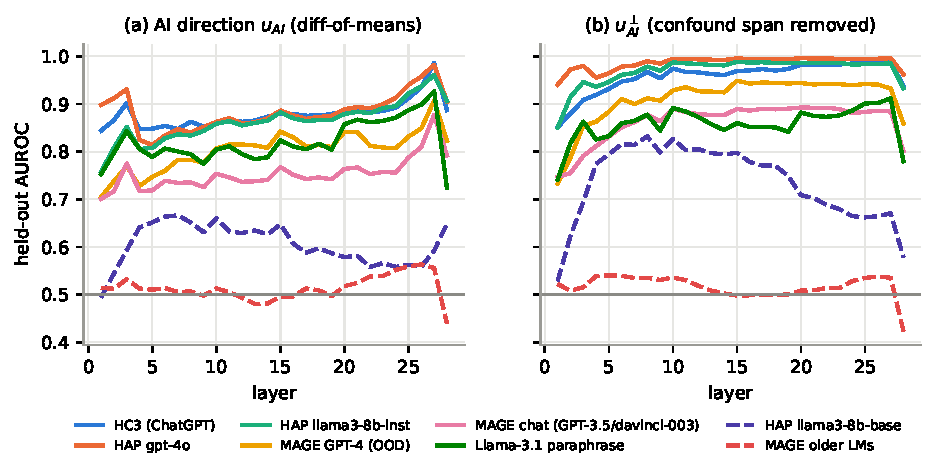
\includegraphics[width=\linewidth]{figures/readout_layers.pdf}
\caption{Held-out AUROC across layers (instruct model). Dashed lines are machine text \emph{not} from chat-tuned models (Llama-3 base continuations, pre-2022 LMs); the direction does not detect it.}
\label{fig:readout_layers}
\end{figure}

Table~\ref{tab:readout} and Figure~\ref{fig:readout_layers} reproduce the read-out result of prior work under stricter controls. A single diff-of-means direction, fit on length-matched pairs, separates held-out human and chat-model text at every layer. AUROC is 0.83--0.86 in the middle layers and up to 0.98 at layer 27. The full probe reaches 0.93--1.00. The direction transfers to generators and corpora never used for fitting: GPT-4 on MAGE (0.81 at L12, 0.91 at L27) and GPT-3.5/davinci-003 (0.74/0.88). It also transfers to Llama-3.1 \emph{paraphrases} of the very human passages they are compared with (0.79/0.93). There, topic, content and length are held fixed and only the author changes. The HC3 and HAP directions are fit on disjoint corpora (Q\&A vs.\ six prose genres) and different generators. They agree substantially (cosine 0.56 at L12; Figure~\ref{fig:cosines}), which supports a shared component across settings~\citep{quaremba2026linear}.

\textbf{What the direction does \emph{not} detect} is informative. Continuations written by Llama-3 \emph{base} models are matched to the same human prefixes as the instruct continuations. They score only 0.59--0.63, against 0.83--0.86 for Llama-3-Instruct. Text from older, pre-chat LMs (OPT, FLAN-T5, LLaMA-1, GPT-J, \dots) is at chance (0.49). Even the full probe is at chance on older LMs (0.51). It reaches 0.85--0.88 on base-model text, but that is close to what per-token NLL alone achieves (0.87--0.91). The direction therefore encodes the style of \emph{chat-tuned} models, not ``machine authorship''. That supports reading it as ``sounds like an AI assistant''.

\subsection{Disentanglement: half confound, but the signal survives removing the confounds}
\label{sec:disentangle}

\begin{figure}[t]
\centering
\begin{minipage}{0.48\linewidth}
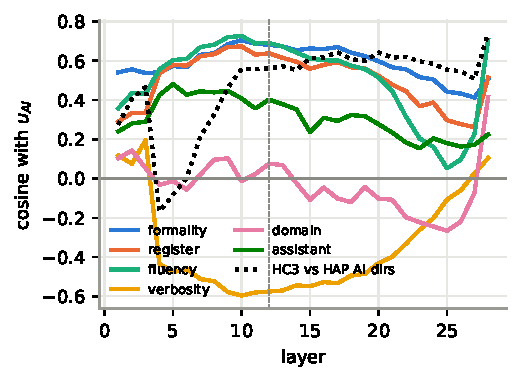
\includegraphics[width=\linewidth]{figures/readout_cosines.pdf}
\end{minipage}\hfill
\begin{minipage}{0.5\linewidth}
\caption{Cosine between $u_{AI}$ and the confound directions across layers (instruct). The dashed vertical line marks the steering layer (12). Each confound direction holds authorship fixed. The dotted line is the agreement between the AI directions fit on HC3 and on HAP. For reference, two random directions in $\mathbb{R}^{3584}$ have $|\cos|\approx 0.02$, and the domain direction stays near 0.}
\label{fig:cosines}
\end{minipage}
\end{figure}

\paragraph{Geometry.} At layer 12, $u_{AI}$ has cosine $0.68$ with formality, $0.69$ with fluency (low NLL), $0.64$ with register, $-0.58$ with verbosity and $0.40$ with the Assistant axis. Its cosine with Reddit-vs-encyclopedic domain is near zero (0.08) (Figure~\ref{fig:cosines}). Projecting $u_{AI}$ onto the 6-dimensional confound span captures 54\% of its squared norm at L12 and 25\% at L27. So the raw direction is roughly half ``formal, fluent, non-verbose, assistant-like'' text. It is clearly \emph{not} the Assistant axis, which it overlaps only moderately and less at late layers ($0.17$ at L27).

\paragraph{The signal is not in the confounds.} Removing the whole confound span and refitting \emph{raises} held-out AUROC at L12, from 0.88--0.91 to 0.97--0.99 on matched sets and from 0.85 to 0.88 on MAGE GPT-4 (Table~\ref{tab:readout}, ``confounds''). Removing a random 6-dimensional subspace changes nothing. The confound-orthogonal direction $u_{AI}^{\perp}$ alone reads out at 0.97--0.99 on matched sets and 0.93 on MAGE GPT-4, far above any single confound direction ($\leq 0.80$). The confounds were mostly adding variance unrelated to authorship. Removing $u_{AI}$ itself and refitting drops AUROC to 0.34--0.71. Much of the linearly decodable signal is concentrated in this one direction, though not all of it (cf.\ INLP~\citep{ravfogel2020null}).

\paragraph{Perplexity.} Perplexity is the strongest scalar confound. AI text is much more likely under Qwen (mean-NLL AUROC 0.79--0.98 on matched sets), and at L12 the raw $u_{AI}$ projection correlates with NLL ($\rho\approx-0.5$ within class). A logistic model on [NLL, length] does not improve when the raw $u_{AI}$ projection at L12 is added (Table~\ref{tab:scalar}; e.g.\ HC3 0.89$\rightarrow$0.90). At this layer the raw direction's read-out is therefore largely a perplexity read-out. The confound-orthogonal $u_{AI}^{\perp}$ behaves differently. It adds substantial information beyond NLL and length (HC3 0.89$\rightarrow$0.98, MAGE GPT-4 0.80$\rightarrow$0.95, content-matched paraphrases 0.68$\rightarrow$0.89), and it keeps AUROC 0.69--0.85 on chat-model text even after NLL and length are regressed out of the projection. Low perplexity is part of what makes text ``sound like AI'', but it is not the whole of what the representation encodes.

\begin{table}[t]
\centering\small
\caption{Scalar confounds at L12 (instruct). AUROC of a logistic model on [mean NLL, log length], with and without the projection on the direction, fit on one half of each eval set and tested on the other. ``Resid.'' is the AUROC of the projection after linearly regressing out NLL and length.}
\label{tab:scalar}
\begin{tabular}{lcccccc}
\toprule
& \multicolumn{3}{c}{$u_{AI}$} & \multicolumn{3}{c}{$u_{AI}^{\perp}$}\\
\cmidrule(lr){2-4}\cmidrule(lr){5-7}
Eval set & NLL+len & +proj & resid. & NLL+len & +proj & resid.\\
\midrule
\tabinput{tables/scalar.tex}
\bottomrule
\end{tabular}
\end{table}

\subsection{Causal test: subtracting the direction makes the model's own answers read as human}
\label{sec:steer}

\begin{table}[t]
\centering\small
\caption{Steering Qwen2.5-7B-Instruct at layer 12, on 160 held-out HC3 questions. Detector and judge columns are means over \emph{English} outputs (\% non-English is the share removed; see text). ``@50w'' = detectors on the first 50 words only, dropping shorter answers (length control). Bino = Binoculars $-B$ (higher = more AI). logit = mean desklib logit, which stays informative where probabilities saturate. Coh./Rel. = Gemma-3 judge, 1--10. Sim = embedding cosine to the unsteered answer to the same question. All control vectors have the same norm as $u_{AI}$ at the same $\alpha$.}
\label{tab:steer}
\setlength{\tabcolsep}{2.6pt}
\begin{tabular}{lrcccccccccr}
\toprule
& \%non- & \multicolumn{2}{c}{P(AI)} & \multicolumn{2}{c}{P(AI) @50w} & & desklib & & & & \\
\cmidrule(lr){3-4}\cmidrule(lr){5-6}
Condition & Engl. & desklib & fakespot & desklib & fakespot & Bino & logit & Coh. & Rel. & Sim & words\\
\midrule
\tabinput{tables/steering.tex}
\bottomrule
\end{tabular}
\end{table}

\begin{figure}[t]
\centering
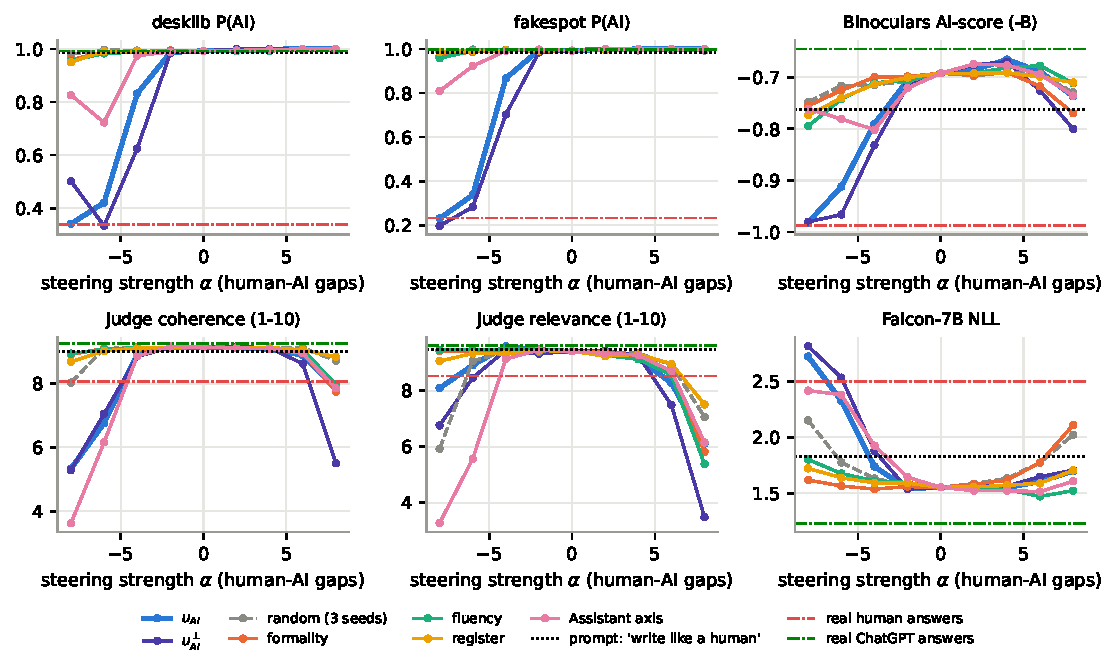
\includegraphics[width=\linewidth]{figures/steering_dose.pdf}
\caption{Dose-response of steering at layer 12, with English outputs only. Negative $\alpha$ pushes towards ``human''. Horizontal lines are the unsteered model's prompt baseline and the real human and ChatGPT answers to the same questions. All directions have equal norm at each $\alpha$.}
\label{fig:dose}
\end{figure}

\begin{table}[t]
\centering\small
\caption{Validation of the independent measures on held-out \emph{real} text: AUROC for separating AI from human text (250 HC3 question pairs; 150 HAP prefixes per generator). The supervised detectors and Binoculars are valid. The Gemma-3 judge's AI-likeness rating is not.}
\label{tab:validation}
\begin{tabular}{lccccc}
\toprule
Contrast & desklib & fakespot & Binoculars & HC3-RoBERTa & judge AI-likeness\\
\midrule
\tabinput{tables/validation.tex}
\bottomrule
\end{tabular}
\end{table}

\paragraph{Validity of the measures.} Before steering we checked every measure on held-out real text (Table~\ref{tab:validation}). Both supervised detectors and Binoculars separate human from AI text almost perfectly (AUROC 0.90--1.00), including base-model text. The Gemma-3-12B judge's AI-likeness rating is near chance (0.46--0.60). It also rates degenerate text as maximally AI-like (Table~\ref{tab:steer_full} in the appendix). We therefore do \textbf{not} use the judge for AI-ness. We keep it only for coherence and relevance, for which it behaves sensibly (unsteered 9.1/9.4; real human answers 8.1/8.5; broken text 1.0). This agrees with the warning in the task framing that LLM judges are noisy on ``sounds like AI''.

\paragraph{Steering towards ``human'' works, and controls do not.} Table~\ref{tab:steer} and Figure~\ref{fig:dose} summarise the results. The unsteered model is detected as AI on essentially every answer (desklib 0.99, fakespot 0.99). Subtracting $u_{AI}$ lowers both supervised detectors and Binoculars, monotonically in $|\alpha|$. At $\alpha{=}{-}6$, mean P(AI) is 0.42 (desklib) and 0.34 (fakespot), and Binoculars moves most of the way from the model ($-0.69$) to real human answers ($-0.99$). The real human answers to the same questions score 0.34/0.23/$-0.99$. Three random directions of identical norm leave the detectors at 0.98--1.00 at every $\alpha$ (paired Wilcoxon $p<10^{-16}$ vs.\ $u_{AI}$ for every detector at $\alpha\leq{-}4$). So did the formality, register and fluency directions (desklib 0.95--0.96 at $\alpha{=}{-}8$) and the Assistant axis (0.72--0.83), even though each of them shares 0.4--0.7 cosine with $u_{AI}$.
\textbf{Length is not the explanation.} Steered answers are shorter, but on only the first 50 words the effect remains (desklib/fakespot 0.69/0.59 at $\alpha{=}{-}6$ and 0.47/0.29 at $\alpha{=}{-}8$, against 0.97/0.95 unsteered and 0.49/0.30 for real human answers).
\textbf{Positive steering} is at the probability ceiling. In logit space it still pushes beyond the unsteered model (desklib logit 8.8 $\rightarrow$ 11.7 at $\alpha{=}{+}8$; random 9.8, formality 9.9). It nearly triples the rate of stock assistant phrases (1.3 $\rightarrow$ 3.4 per 100 words), producing text such as ``\emph{Navigating the landscape of financial challenges can be complex\ldots}''.

\paragraph{Coherence cost and matched-quality comparison.} The effect costs some quality. At $\alpha{=}{-}4$ judge coherence falls only from 9.1 to 8.9, and relevance even rises (9.6), but the detectors only reach 0.83/0.87. At $\alpha{=}{-}6$ coherence is 6.8 (real human answers: 8.1). Two observations show the detector shift is not a by-product of degradation. First, equal-norm random directions at $\alpha{=}{-}8$ degrade coherence comparably (7.6--8.7) without moving the detectors. Second, Table~\ref{tab:matched} keeps only answers the judge rates $\geq 8$ on \emph{both} coherence and relevance. Among these high-quality answers, $u_{AI}$ at $\alpha{=}{-}6$ still scores 0.53/0.42 and $u_{AI}^{\perp}$ scores 0.40/0.30, which matches real human answers that pass the same filter (0.36/0.26). Random and confound directions stay at 0.96--1.00. Figure~\ref{fig:tradeoff} shows the whole frontier: at every coherence level, $u_{AI}$ and $u_{AI}^{\perp}$ dominate all controls.

\paragraph{The confound-orthogonal component is the better steering vector.} $u_{AI}^{\perp}$ has no component along formality, register, fluency, verbosity, domain or the Assistant axis. It steers \emph{at least as well} as $u_{AI}$ (desklib 0.62 vs.\ 0.83 at $\alpha{=}{-}4$, at equal coherence 8.8--8.9; 0.33 vs.\ 0.42 at $\alpha{=}{-}6$), and it almost never switches language (1\% vs.\ 13\% at $\alpha{=}{-}6$). The causal effect on detectors therefore does not run through the measured confounds.

\paragraph{The prompt baseline barely moves the detectors.} Asking the model to answer ``like an ordinary person on Reddit, not like an AI'' changes the surface: ``Hey there!'', fewer lists, more contractions. But detectors still flag 99\% of answers (desklib 0.99, fakespot 0.98, Binoculars $-0.76$). Prompt plus steering ($\alpha{=}{-}4$) reaches 0.68/0.60 at coherence 7.8, slightly better than steering alone at that coherence. The direction captures something the model does not change when merely instructed to sound human.

\paragraph{What changes in the text.} Under negative steering, answers lose markdown lists and stock assistant phrases (``it is important to'', ``generally'', ``consult''; 1.3 $\rightarrow$ 0.4 per 100 words at $\alpha{=}{-}6$). They also get shorter, more direct and more first-person (Figure~\ref{fig:style} and Table~\ref{tab:examples} in the appendix). Content is largely preserved at moderate strength. The embedding similarity to the unsteered answer is 0.84 at $\alpha{=}{-}4$ and 0.78 at $\alpha{=}{-}6$, against 0.91 between two unsteered samples with different seeds and 0.67 between the model's answer and the real human answer.

\paragraph{Failure modes.} (i)~\emph{Language switching}: strong negative steering with $u_{AI}$ sometimes makes the model answer in Chinese (3\% at $\alpha{=}{-}4$, 13\% at $-6$, 38\% at $-8$). The fluency direction does this too (22\% at $-8$). English-trained detectors are not valid on such text, so all reported numbers exclude these outputs. With them included, the detector scores are similar or lower (Appendix~\ref{app:full}). That $u_{AI}^{\perp}$ rarely switches language suggests the switching runs through the fluency/low-NLL component: for Qwen, much of its most ``fluent'' mass may be Chinese.
(ii)~\emph{Multi-layer interventions are brittle}. Adding $\alpha g_\ell u_{AI,\ell}$ at all 27 layers works at $\alpha{=}{-}0.25$ (desklib 0.71 at coherence 7.2). At $|\alpha|\geq 0.5$ it destroys coherence. Clamping every token's projection to the human mean at all layers (a directional ablation) produces gibberish (coherence 1.1). The direction is defined by \emph{mean-pooled} statistics, and forcing every token to the pooled mean is far outside the data distribution.

\begin{table}[t]
\centering\small
\caption{Matched-quality comparison: mean detector P(AI) over English answers that the judge rates $\geq8$ for \emph{both} coherence and relevance, and the share of answers that pass the filter.}
\label{tab:matched}
\setlength{\tabcolsep}{3.2pt}
\begin{tabular}{lccccccccc}
\toprule
& \multicolumn{3}{c}{$\alpha{=}{-}4$} & \multicolumn{3}{c}{$\alpha{=}{-}6$} & \multicolumn{3}{c}{$\alpha{=}{-}8$}\\
\cmidrule(lr){2-4}\cmidrule(lr){5-7}\cmidrule(lr){8-10}
Direction & desklib & fakespot & kept & desklib & fakespot & kept & desklib & fakespot & kept\\
\midrule
\tabinput{tables/matched_quality.tex}
\bottomrule
\end{tabular}
\end{table}

\begin{figure}[t]
\centering
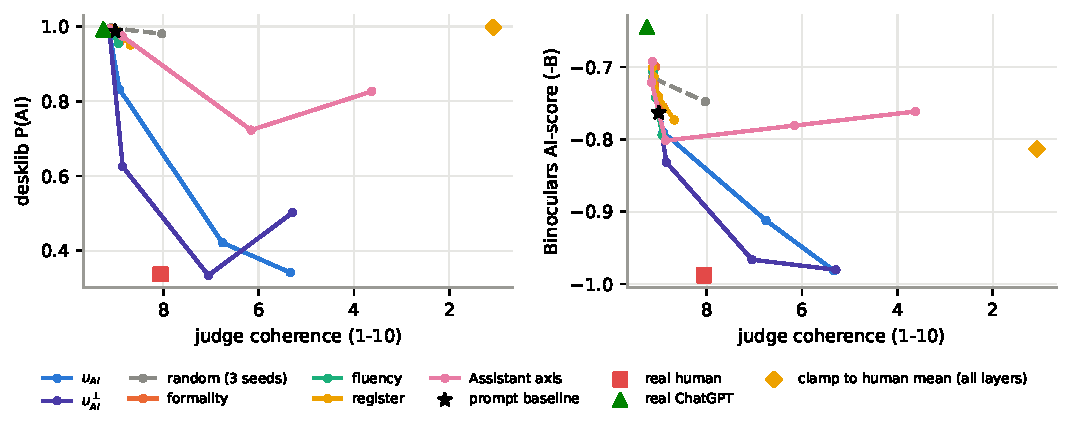
\includegraphics[width=\linewidth]{figures/steering_tradeoff.pdf}
\caption{Detector score vs.\ judge coherence for each steering family as $|\alpha|$ grows (negative $\alpha$; the curves start at the unsteered model, top left). Lower and further left is better. Markers show the prompt baseline, real human and ChatGPT answers, and all-layer clamping.}
\label{fig:tradeoff}
\end{figure}

\subsection{Base vs.\ instruct: the direction predates chat tuning}
\label{sec:base}

\begin{figure}[t]
\centering
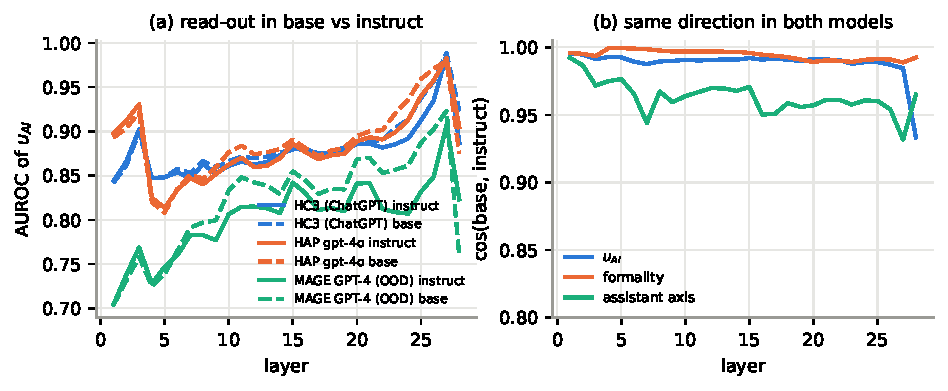
\includegraphics[width=\linewidth]{figures/base_vs_instruct.pdf}
\caption{(a) Read-out AUROC of $u_{AI}$ fit separately in the base (dashed) and instruct (solid) model. (b) Cosine between the base and instruct versions of $u_{AI}$, the formality direction and the Assistant axis, at each layer.}
\label{fig:base}
\end{figure}

We repeated the read-out in the pretrained Qwen2.5-7B, fitting all directions afresh from its own activations. The AI direction in the base model is nearly identical to the instruct one: cosine 0.98--0.995 at every layer from 1 to 27 (Figure~\ref{fig:base}b). Its read-out AUROC is equal or slightly higher, by 0.005--0.018 on average across layers. The base direction applied to instruct activations reads out as well as the instruct direction (0.87 vs.\ 0.86 on HC3 at L12). Chat tuning therefore neither created nor measurably amplified the representation \emph{of} AI-sounding text. The Assistant axis is also largely shared (cosine $\geq0.93$), as \citet{lu2026assistant} report. One caveat: Qwen2.5's pretraining data postdates ChatGPT and likely contains AI-written text, so ``base'' does not mean ``never saw AI text''.

The base direction is also causal in the base model (Table~\ref{tab:base}). We continue 160 held-out human text prefixes from HAP. Desklib already flags unsteered Qwen base continuations as AI (0.97). Subtracting $u_{AI}^{base}$ lowers this to 0.63 ($\alpha{=}{-}4$) and 0.43 ($\alpha{=}{-}8$), while an equal-norm random direction does not (0.96/0.94). Adding it makes continuations of human fiction and news sound like an assistant: the stock-phrase rate rises ninefold (0.22 $\rightarrow$ 1.99 per 100 words) and the desklib logit rises from 5.7 to 11.7 (random: 7.6). One example continues a Victorian children's story with ``\emph{Together, they spent countless hours exploring the world\ldots\ Despite the challenges that life presented, the child grew stronger and more resilient}''. So the pretrained model already has a steerable ``assistant voice'', which chat tuning then makes the default.

\begin{table}[t]
\centering\small
\caption{Steering the \emph{base} model (Qwen2.5-7B) with its own $u_{AI}$ at L12, continuing 160 human text prefixes. AI-phr = stock assistant phrases per 100 words. Coh. = judge coherence.}
\label{tab:base}
\begin{tabular}{lccccccc}
\toprule
Condition & desklib & fakespot & Bino & desklib logit & AI-phr & Coh. & words\\
\midrule
\tabinput{tables/base_steering.tex}
\bottomrule
\end{tabular}
\end{table}
